%%%%%%%%%%%%%%%%%%%%%%%%%%%%%%%%%%%%%%%%%%%%%%%%%%%%
%												   %
%  BIBLIOTECA									   %
%												   %
%  Janeiro 2015								       %
%												   %
%  Angela Cardoso, Catarina Terra e Maria Miranda  %
%   											   %	
%%%%%%%%%%%%%%%%%%%%%%%%%%%%%%%%%%%%%%%%%%%%%%%%%%%%

\documentclass[12pt,a4paper,reqno]{report}
\linespread{1.5}

\usepackage{amsfonts,amsmath,amssymb,indentfirst,mathrsfs,amscd}
\usepackage[mathscr]{eucal}
\usepackage[active]{srcltx} %inverse search
\usepackage{tensor}
\usepackage[utf8x]{inputenc}
\usepackage[portuges]{babel}
\usepackage[T1]{fontenc}
\usepackage{tikz}
\usepackage{graphicx}
\usepackage[numbers,square, comma, sort&compress]{natbib}
\numberwithin{figure}{section}
\numberwithin{equation}{section}
\usepackage{scalefnt}
\usepackage[top=2.5cm, bottom=2.5cm, left=2.5cm, right=2.5cm]{geometry}
\usepackage{comment} 
%\usepackage{tweaklist}
%\renewcommand{\itemhook}{\setlength{\topsep}{0pt}%
%	\setlength{\itemsep}{0pt}}
%\renewcommand{\enumhook}{\setlength{\topsep}{0pt}%
%	\setlength{\itemsep}{0pt}}
%\usepackage[colorlinks]{hyperref}
\usepackage{MnSymbol}
%\usepackage[pdfpagelabels,pagebackref,hypertexnames=true,plainpages=false,naturalnames]{hyperref}
\usepackage[naturalnames]{hyperref}
\usepackage{enumitem}
\usepackage{titling}
\newcommand{\subtitle}[1]{%
  \posttitle{%
    \par\end{center}
    \begin{center}\large#1\end{center}
    \vskip0.5em}%
}
\newcommand{\HRule}{\rule{\linewidth}{0.5mm}}

\usepackage[official]{eurosym}

\def\Cpp{C\raisebox{0.5ex}{\tiny\textbf{++}}}

\makeatletter
\def\@makechapterhead#1{%
  %%%%\vspace*{50\p@}% %%% removed!
  {\parindent \z@ \raggedright \normalfont
    \ifnum \c@secnumdepth >\m@ne
        \huge\bfseries \@chapapp\space \thechapter
        \par\nobreak
        \vskip 20\p@
    \fi
    \interlinepenalty\@M
    \Huge \bfseries #1\par\nobreak
    \vskip 40\p@
  }}
\def\@makeschapterhead#1{%
  %%%%%\vspace*{50\p@}% %%% removed!
  {\parindent \z@ \raggedright
    \normalfont
    \interlinepenalty\@M
    \Huge \bfseries  #1\par\nobreak
    \vskip 40\p@
  }}
\makeatother


\begin{document}

\input{./title.tex}

\tableofcontents

%%%%%%%%%%%%%%
% INTRODUCAO %
%%%%%%%%%%%%%%
\chapter{Introdução}

No âmbito da disciplina de Algoritmos e Estruturas de Dados, foi-nos proposto implementar em \Cpp{} uma aplicação que permita a gestão de uma biblioteca. Entretanto, como segunda parte desse trabalho, alteramos e acrescentamos novas estruturas, de forma a permitir a manutenção de pedidos de empréstimo, de leitores inativos e de livros disponíveis.

O sistema inicial continha informações sobre livros, leitores, funcionários e empréstimos de livros. A aplicação permitia registar e gerir os empréstimos efetuados na biblioteca, assim como toda a informação já referida. Entretanto, adicionaram-se três novas estruturas à biblioteca: uma árvore binária de pesquisa com os livros disponíveis para emprestar; uma tabela de dispersão com os leitores inativos, que não efetuam empréstimos há mais de um ano; uma fila de prioridade com os pedidos de empréstimo dos livros indisponíveis.

Mantiveram-se as restrições anteriores. Cada leitor não pode ter mais de 3 livros emprestados em simultâneo. Por casa dia de atraso o leitor incorre numa multa. Um livro pode ser emprestado por um período máximo de 1 semana ou não pode ser emprestado. Cada empréstimo é feito por um funcionário. Os funcionários podem ou não ser supervisores e cada supervisor é responsável por um ou mais funcionários, nunca por outro supervisor, devendo esta distribuição ser equilibrada.

Os livros passam a ter informação sobre o ano de edição, estando os livros disponíveis ordenados na árvore por ano de edição, título e autores.

Os pedidos estão ordenados por data e, em caso de serem do mesmo dia, por prioridade dos leitores, estudantes primeiro, depois crianças e finalmente adultos.

Ao longo deste documento descreve-se a aplicação que desenvolvemos para gestão de um biblioteca, com foco nos desenvolvimentos da segunda parte do trabalho.

%%%%%%%%%%%%%
% DESCRICAO %
%%%%%%%%%%%%%
\chapter{Descrição da Solução Implementada}

Para conter toda a informação de uma biblioteca, implementou-se a classe \textbf{Biblioteca}, que é constituída pelas seguintes estruturas:
\begin{itemize}
\item \textit{livros} - vetor com todos os livros da biblioteca;
\item \textit{funcionarios} - vetor com todos os funcionários, incluindo os supervisores e o administrador;
\item \textit{leitores} - vetor com todos os leitores da biblioteca;
\item \textit{emprestimos} - vetor com todos os empréstimos da biblioteca;
\item \textit{pedidos} - vetor com todos os pedidos de empréstimo da biblioteca;
\item \textit{disponiveis} - árvore binária de pesquisa com os livros disponíveis para empréstimo;
\item \textit{inativos} - tabela de dispersão com os leitores inativos há mais de um ano;
\item \textit{utilizadores} - vetor com todos os utilizadores do sistema informático da biblioteca.
\end{itemize}

Com exceção dos utilizadores, quando um objeto é removido (por exemplo, no caso de devolução de um empréstimo), não desaparece, apenas é alterado para indicar que já não existe, sendo-lhe acrescentada a data de remoção. Assim, para a classe \textbf{Livro} (respectivamente, \textbf{Funcionario}, \textbf{Leitor}, \textbf{Emprestimo}, \textbf{Pedido}) existe a subclasse \textbf{Livro\_old} (respectivamente, \textbf{Funcionario\_old}, \textbf{Leitor\_old}, \textbf{Emprestimo\_old}, \textbf{Pedido\_old}), para onde é enviado um livro (respectivamente, funcionário, leitor, empréstimo) quando é removido.

As classes \textbf{Livro}, \textbf{Funcionario}, \textbf{Leitor}, \textbf{Emprestimo}, \textbf{Pedido} e \textbf{Utilizador} são subclasses da classe \textbf{Object}, que tem como único atributo o código de identificação \textbf{ID}.

O primeiro passo na utilização da aplicação é efetuar o login. Para isso é necessário indicar o ID e a password, sendo então determinado o tipo de acesso do utilizador, 0 se for administrador (gerente da biblioteca), 1 se for um supervisor e 2 se for um funcionário. \underline{ID}, \underline{password} e \underline{acesso} são atributos da classe \textbf{Utilizador}.

Uma das funções mais procuradas numa biblioteca é o empréstimo de livros a leitores. A classe \textbf{Emprestimo} faz a gestão dessas funções e tem como parâmetros um apontador para o livro do emprestimo, um apontador para o funcionario que fez o emprestimo, um apontador para o leitor do emprestimo, a data do emprestimo e um contador de emprestimos feitos na biblioteca (atuais e antigos).

Não estando nenhum exemplar do livro disponível para empréstimo, é possível deixar um pedido de empréstimo. A classe \textbf{Pedido} faz a gestão dessas funções e tem como parâmetros um apontador para o livro do pedido, um apontador para o funcionario que fez o pedido, um apontador para o leitor do pedido, a data do pedido e um contador de pedidos feitos na biblioteca (atuais e antigos). Além de serem mantidos num vetor na biblioteca, os pedidos são mantidos em filas de prioridade dos respetivos livros, uma vez que quando são de livros distintos, não há qualquer relação de prioridade entre dois pedidos.

Quando se tenta adicionar um empréstimo e o livro não está disponível, é possível adicionar um pedido. Além disso, ao devolver um livro para o qual haja pedidos, é possível transformar o pedido mais prioritário num novo empréstimo. Em qualquer caso, mesmo que não seja feito o empréstimo, o pedido é removido, considerando-se que o leitor desistiu. 

Tal como as classes \textbf{Emprestimo} e \textbf{Pedido}, as classes \textbf{Livro}, \textbf{Funcionario} e \textbf{Leitor}, também possuem contadores do numero dos seus objetos na biblioteca. Estes contadores são utilizados para permitir a atribuição automática de códigos de identificação a cada um destes objetos. Assim, se adicionamos um novo livro à biblioteca, por exemplo, e em toda a sua existência (atuais e antigos) a biblioteca teve 13 livros, o ID do novo livro será 14.

A classe \textbf{Livro} tem como atributos o \underline{ano\_edicao}, o \underline{titulo}, um vetor com os nomes dos \underline{autores}, o \underline{tema}, o \underline{ISBN}, a \underline{cota} do livro na biblioteca, o \underline{num\_paginas}, a \underline{edicao}, o número de \underline{exemplares} desse livro, o número \underline{ex\_disponiveis} de exemplares que estão disponíveis para emprestar e um vetor \underline{emp\_livro} com apontadores para os empréstimos de cada exemplar do livro. Sendo assim, cada exemplar corresponde a um índice do vetor de empréstimos e, se o exemplar estiver disponível, no respetivo índice do vetor está um apontador nulo.

Além dos atributos já referidos, o único atributo da classe \textbf{Funcionario} é o \underline{nome} do funcionário. A classe \textbf{Supervisor} é subclasse de \textbf{Funcionario} e tem como atributo adicional um vetor \underline{funcionarios\_sup} de apontadores para os funcionários supervisionados pelo supervisor. Uma vez que o número de funcionários supervisionados por cada supervisor deve ser equilibrado, a distribuição dos funcionários pelos supervisores é feita de forma automática, garantindo o equilíbrio, de cada vez que:
\begin{itemize}
	\item é adicionado um funcionário;
	\item é removido um funcionário ou supervisor;
	\item é promovido um funcionário a supervisor;
	\item é despromovido um supervisor a funcionário.
\end{itemize}

Existe ainda a classe \textbf{Administrador}, como subclasse de \textbf{Funcionario} (sem atributos adicionais). Apenas é adicionado um administrador à biblioteca, com o ID 0 e o nome Administrador. Este age como gerente da biblioteca, sendo o único que tem acesso total e que pode adicionar, remover, promover e despromover funcionários. É também o único que pode efetuar a manutenção dos utilizadores.

Além dos mencionados acima, os atributos da classe \textbf{Leitor} são o \underline{nome}, o \underline{tipo} (estudante, criança ou adulto), o \underline{telefone}, o \underline{email} e um vetor \underline{emprestimos\_leitor} com apontadores para os seus empréstimos.

A interação do utilizador com a aplicação é feita primariamente através de uma série de menus na consola, de seleção numérica. Uma sequência de opções nestes menus, conduz a uma função da classe \textbf{Biblioteca}, que por sua vez poderá chamar uma ou mais funções das restantes classes mencionadas. A gestão destes menus é feita na classe \textbf{Menu}, subclasse de \textbf{Biblioteca}, que como atributo adicional tem um \textbf{Utilizador\_online}, consoante o qual é determinado o tipo de acesso e as funções disponíveis.

Além das classes mencionadas, existem ainda várias classes onde estão parametrizadas as exceções a usar quando não existe um determinado objeto, tentamos adicionar um empréstimo a um leitor com 3 empréstimos, tentamos emprestar um livro já emprestado, tentamos pedir um livro disponível, tentamos remover um objeto ocupado (livro emprestado, por exemplo), tentamos utilizar um ficheiro que não existe, etc.

%%%%%%%%%%%%
% DIAGRAMA %
%%%%%%%%%%%%
\chapter{Diagrama de Classes UML}

\begin{center}

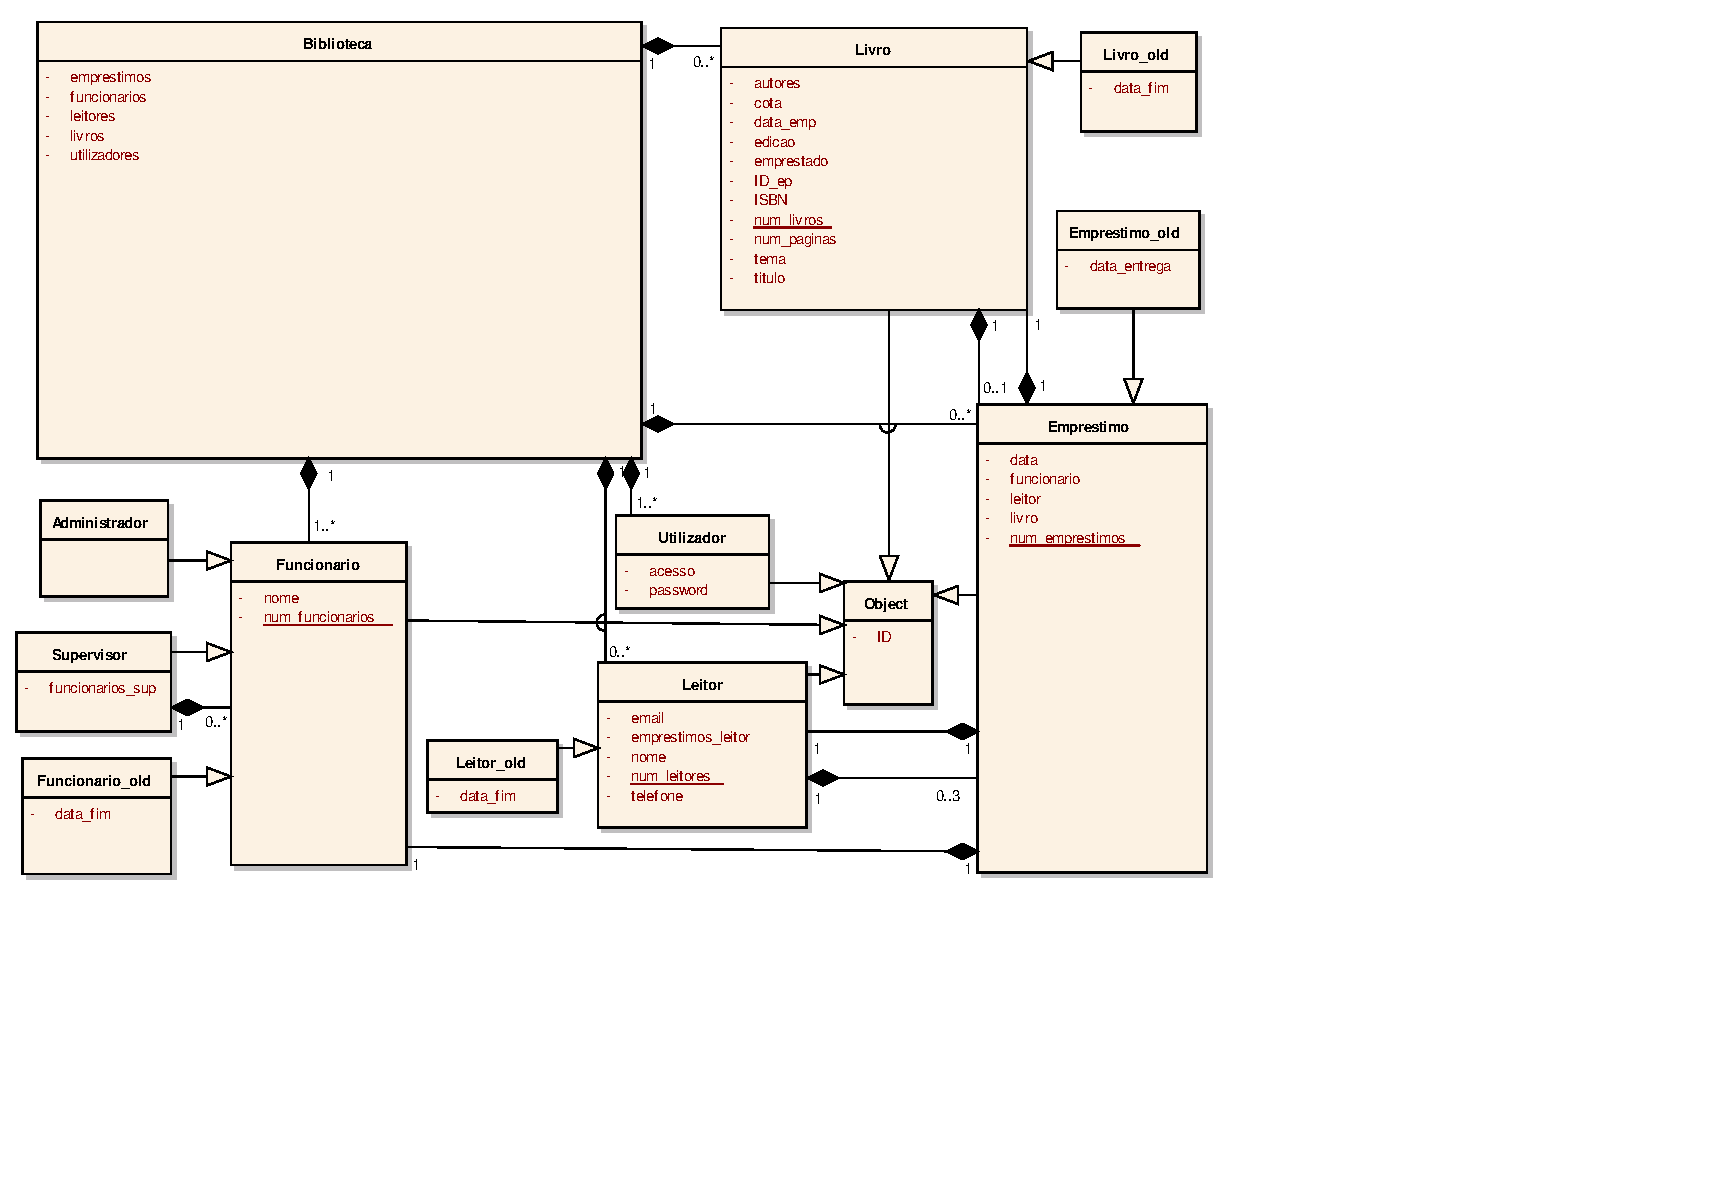
\includegraphics[width=14.4cm]{UML.jpg}

\end{center}

%%%%%%%%%%%%%%
% UTILIZACAO %
%%%%%%%%%%%%%%
\chapter{Casos de Utilização}

A aplicação para gestão de uma biblioteca construída permite registar informaticamente uma série de atividades relacionadas com o funcionamento normal de uma biblioteca.

\begin{enumerate}
  \item Consultas
  \begin{enumerate}[label*=\arabic*.]
    \item Livros
    \item Empréstimos
    \item Pedidos
    \item Leitores
    \item Funcionários
    \item Supervisores
    \item Utilizadores
  \end{enumerate}
  \item Empréstimos
  \begin{enumerate}[label*=\arabic*.]
    \item Adicionar
    \item Devolver
    \item Consultar atrasos
    \item Consultar atrasos por leitor
    \item Consultar livros atrasados
    \item Consultar antigos
  \end{enumerate}
  \item Pedidos
  \begin{enumerate}[label*=\arabic*.]
    \item Adicionar
    \item Desistir
    \item Consultar antigos
  \end{enumerate}
  \item Livros
  \begin{enumerate}[label*=\arabic*.]
    \item Consultar disponíveis
    \item Consultar emprestados
    \item Consultar por tema
    \item Consultar antigos
    \item Adicionar
    \item Remover
    \item Alterar
	\begin{enumerate}[label*=\arabic*.]
		\item Ano de edição
		\item Título
		\item Autores
		\item Tema
		\item ISBN
		\item Cota
		\item Número de páginas
		\item Edição
		\item Tudo
	\end{enumerate}
  \end{enumerate}
  \item Leitores
  \begin{enumerate}[label*=\arabic*.]
    \item Adicionar
    \item Remover
    \item Alterar
	\begin{enumerate}[label*=\arabic*.]
		\item Nome
		\item Tipo
		\item Telefone
		\item Email
		\item ISBN
		\item Morada
		\item Tudo
	\end{enumerate}
	\item Consultar inativos
    \item Consultar antigos
  \end{enumerate}
  \item Funcionários
  \begin{enumerate}[label*=\arabic*.]
    \item Adicionar
    \item Remover
    \item Promover
    \item Despromover
    \item Consultar antigos
  \end{enumerate}
  \item Utilizadores
  \begin{enumerate}[label*=\arabic*.]
    \item Adicionar
    \item Remover
  \end{enumerate}
\end{enumerate}

A disponibilidade destas funções depende do nível de acesso do utilizador. De forma geral, um supervisor pode, além de todas as tarefas acessíveis a um funcionário, adicionar e remover livros e consultar informação sobre funcionários. O administrador é o único que pode fazer a manutenção dos funcionários e dos utilizadores.

%%%%%%%%%%%%%%%%
% DIFICULDADES %
%%%%%%%%%%%%%%%%
\chapter{Principais Dificuldades}

Nesta segunda parte, a maior dificuldade de implementação foi fazer as alterações necessárias ao que já tinha sido feito anteriormente. Além do que se acrescentou, foi preciso fazer várias mudanças às classes \textbf{Livro} e \textbf{Leitor}. Cada alteração teve diversos impactos nas outras classes e nas várias funções. Foi necessário alterar tudo isso e os ficheiros de texto, garantindo que a aplicação continuava a funcionar.

Além disso, surgiram algumas dificuldades relacionadas com o facto de se guardarem objetos na árvore de pesquisa, nas filas de prioridade e na tabela de dispersão, em vez de apontadores como se faz nos vetores. Foi necessário colocar objetos na árvore e nas filas, para que estas respeitassem as respetivas ordens dos elementos. No entanto, isto implicou a adição de passos quando se altera um livro ou um leitor, para garantir que os respetivos elementos da árvore e da tabela de dispersão são alterados também.

De resto, uma vez que todas as ferramentas já são conhecidas e o domínio da própria linguagem também é maior, foi mais simples implementar a segunda parte do trabalho. Entre outras coisas, tivemos oportunidade de melhorar vários pontos daquilo que foi feito anteriormente.

%%%%%%%%%%%%%%%%
% DISTRIBUICAO %
%%%%%%%%%%%%%%%%
\chapter{Distribuição de Trabalho Pelos Elementos do Grupo}

Em relação à primeira parte do trabalho, houve aqui melhorias significativas, nomeadamente a nível de comunicação entre os elementos do grupo.

Embora de forma muito menos acentuada, a disponibilidade dos elementos do grupo para o trabalho continuou a não ser a mesma. Desta forma, a Ângela acabou por realizar a maior parte das tarefas de codificação. A Catarina e a Maria, além de alguma contribuição na codificação e na alteração dos ficheiros de texto, dedicaram-se a validar o funcionamento da aplicação, tendo elaborado e efetuado uma bateria de testes por forma a detectar possíveis erros de codificação.

\chapter{Conclusão}

Pela forma como o trabalho se desenvolveu, além do acumular de conhecimento, cremos que a experiência e o resultado final foram mais positivos nesta segunda parte.

O trabalho manteve-se muito interessante e foi gratificante poder aplicar os conhecimentos adquiridos na parte final da disciplina. Mais uma vez ajudou-nos a sedimentar o conhecimento dos diferentes tipos de estrutura utilizados.

Como sempre, se o tempo o permitisse, certamente seriam várias as alterações e melhorias introduzidas. Mas de uma forma geral estamos satisfeitas com o resultado final.

\end{document}
